\subsection{Sparx Systems Enterprise Architect}
Sparx Systems \entArch~is another tool that provides modeling of UML diagrams.
It supports mind map diagrams and project management, to provide full traceability from requirements specification to deployment end implementation.
This tool also provides some metrics evaluation to compute the complexity of a project based on Use Case diagrams. 

To perform this evaluation, the user needs to provide a level of implementation complexity for each interaction with authors. 
This task can be done when defining the Use Case descriptions or when performing the metrics evaluation.

To evaluate the metrics, \entArch~has a wizard which enables other options for the complexity analysis.
These options manipulate the \emph{Technical} and the \emph{Environment} complexities and are used to adapt the evaluation and perform a better result on estimation.

Also can be filtered the Use Cases used in evaluation. 
To filter can be used manual selection or regular expressions over use case name.
This kind of filtering enables the project to be distributed and evaluated individually.

\subsubsection{Results}
To use this tool in metrics calculation, have the possibility do some tweaking over use case complexity, on their description, to get more precise results.
This complexity admits simple values like low, medium or high.\\
Some factors related to environment and technics complexity coud also be edited or hour rates in the wizard shown on the left side of Figure \ref{img:sparxRes}.
Here we can use multiple factors to evaluate this factors, like usability or portability on technical complexity.\\
In the end we can access the Use Case metrics wizard and it is presented to us, as in the right side in Figure \ref{img:sparxRes}, the set of default
values used to evaluate the effort of task.

\begin{figure}[!htbp]
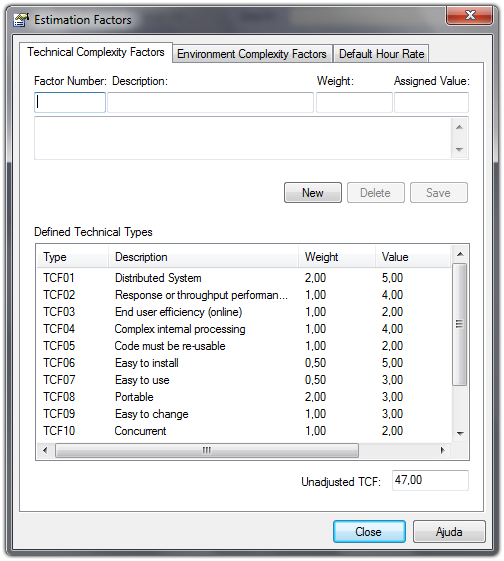
\includegraphics[scale=0.257]{images/sparxestim.png}
\hspace{0.1cm}
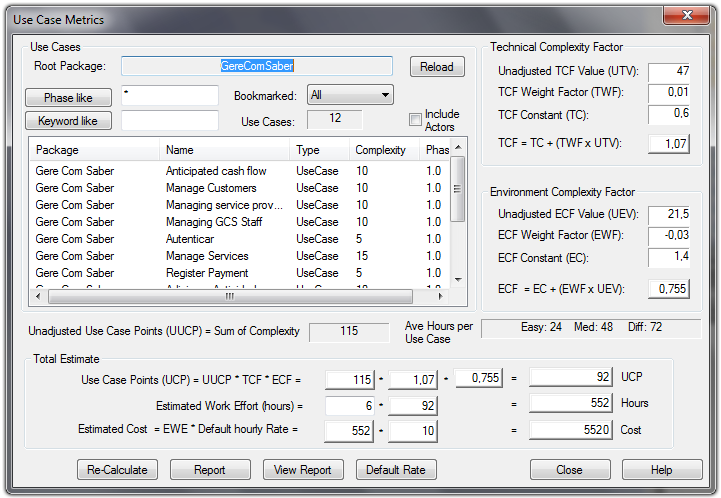
\includegraphics[scale=0.29]{images/sparx.png}
\caption{Estimation Factors and Use Case Metrics \entArch~wizards}\label{img:sparxRes}
\end{figure}

The final result of metrics evaluation, is an estimation of Working Hours, Use Case Points\cite{Ribu01estimatingobject-oriented} and Total Cost needed to perform
the development of system.\\

In Our case, because we have twelve Use Cases and had many of them with medium complexity. The effort to complete the task is 552 working hours, that would give a final result of \EUR{5.520}. 
To get this value only was changed the use cases complexity and everything else was left with default values.
